\chapter{Drag Meta-Modeling}
Drag force comes from many different contributions, but can generally be split into drag that is independent of lift, and drag that is due to lift \cite{nicolaiWhitePaper}. The summation of all sources of drag that are  independent of lift is often called minimum drag ($C_{D_{min}}$ often used for the coefficient)\cite{raymer}, and is roughly constant, for a given Reynold's number and Mach number. The drag due to lift can be split into viscous drag-due-to-lift and inviscid drag-due-to-lift.\\
\begin{figure}[h!]
  \centering
  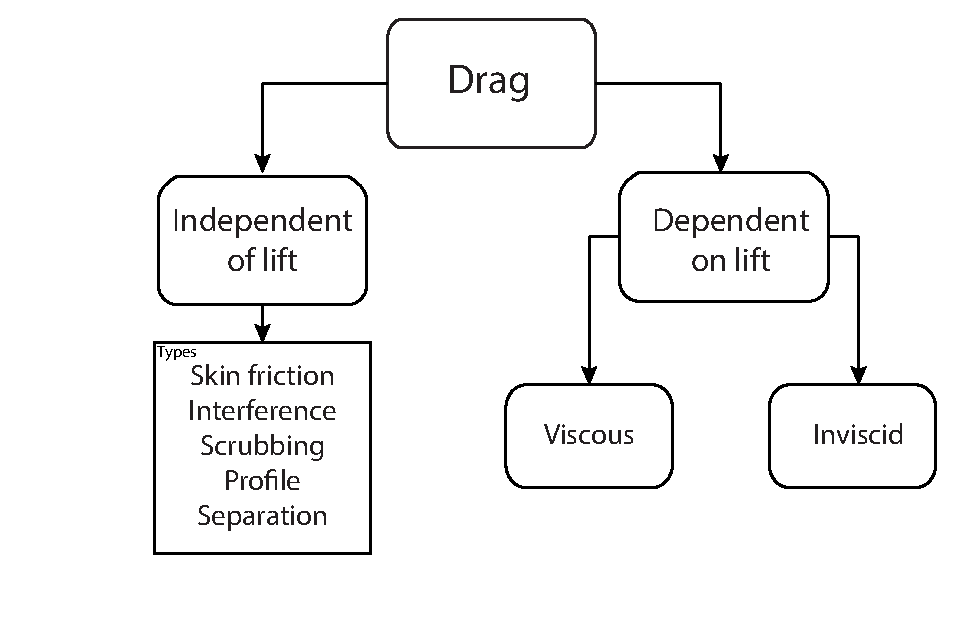
\includegraphics[width=.6\linewidth]{figures/dragDefinition.eps}
  \captionof{figure}{Drag Contribution Types}
  \label{dragDefFig}
\end{figure}

 The viscous drag-due-to-lift is a type pressure drag that increases when the angle of attack of the wing increases, therefore generating more lift. It is a function of airfoil geometry, such as leading edge radius, thickness distribution, and camber. This type of drag is independent of finite wing vortices, and can be seen on two-dimensional airfoil data charts. To show an example of viscous drag-due-to-lift, a NACA 4412 was analyzed using XFOIL\cite{xfoil}.
\begin{figure}[h!]
\centering
\begin{minipage}{.5\textwidth}
  \centering
  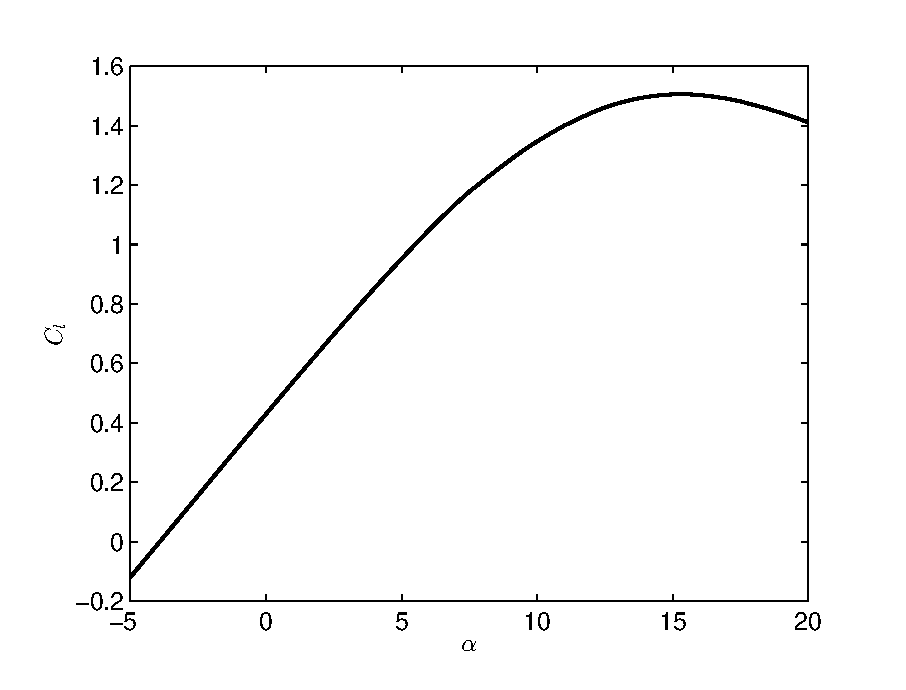
\includegraphics[width=.9\linewidth]{figures/naca4412liftcurve.eps}
  \captionof{figure}{NACA 4412 Lift Curve}
  \label{naca4412liftcurve}
\end{minipage}%
\begin{minipage}{.5\textwidth}
  \centering
  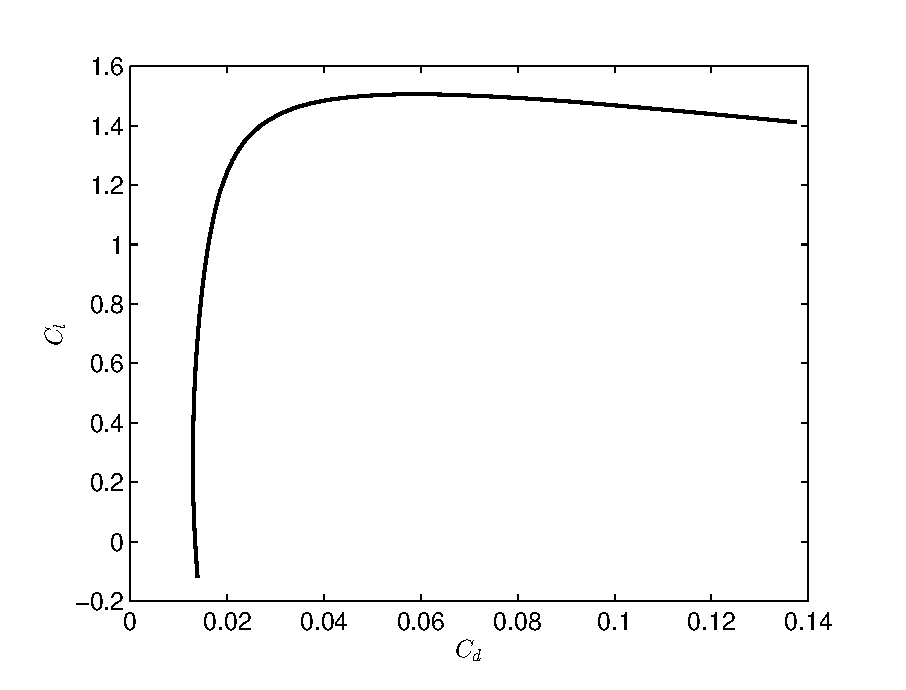
\includegraphics[width=.9\linewidth]{figures/naca4412dragpolar.eps}
  \captionof{figure}{NACA 4412 Drag Polar}
  \label{naca4412dragpolar}
\end{minipage}
\end{figure}

Figure \ref{naca4412dragpolar} shows the airfoils viscous drag-due-to-lift. Since the shape is roughly parabolic through the linear region of the lift curve, the contribution to the total aircraft drag is approximated using the Equation \ref{viscDragDueToLiftEqn}\cite{nicolaiWhitePaper}.
\begin{align}
\label{viscDragDueToLiftEqn}
C_{D_{Visc. Lift}} = K_1 * (C_L - C_{L_{Min Drag}})^2
\end{align}

where $K_1$ is the slope of the line shown in Figure \ref{naca4412cdmin}, and $C_{L_{MinDrag}}$ is the lift coefficient at which minimum drag occurs (roughly 0.25 for this airfoil).

\begin{figure}[h!]
  \centering
  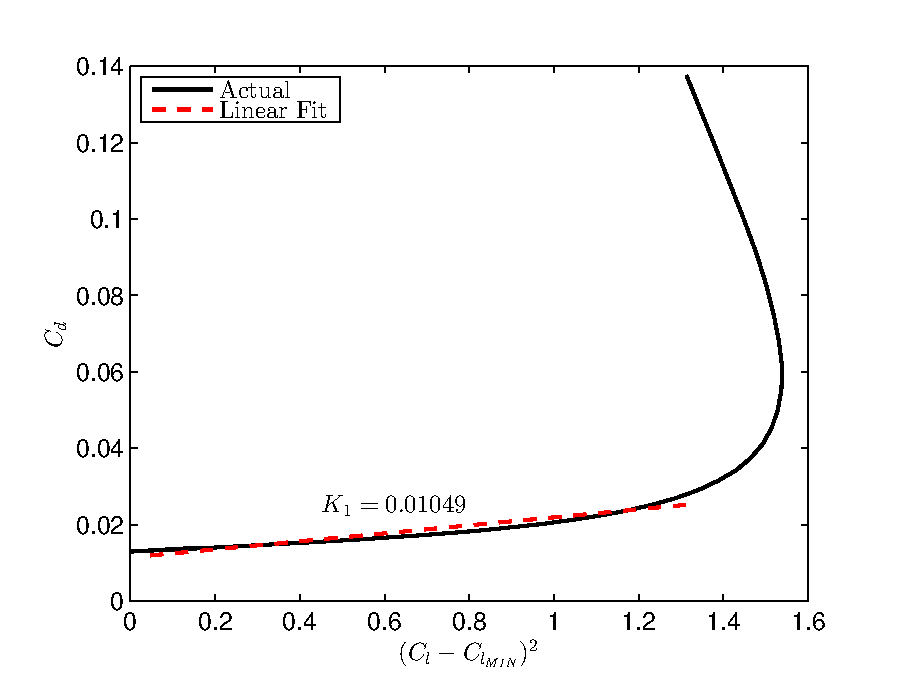
\includegraphics[width=.6\linewidth]{figures/naca4412cdmin.eps}
  \captionof{figure}{NACA 4412 $K_1$ Estimation}
  \label{naca4412cdmin}
\end{figure}
%todo: find a way to estimate K_1 based on curvature (ie which points to take in regression) You can finite difference second derivative, find points where it is close to 0, then take those points and do a linear regression on it.
\textit{Inviscid} drag-due-to-lift occurs because of the pressure difference between the top and bottom of a finite wing. This pressure difference causes the high pressure flow underneath the wing to slip over to the top of the wing, causing a downwash velocity on the free stream velocity, shown in Figure \ref{downwash}.
\begin{figure}[H]
  \centering
  \includegraphics[width=.6\linewidth]{figures/downwash.eps}
  \captionof{figure}{Downwash Caused By Wingtip Vortices\cite{737wingTipVortices}}
  \label{downwash}
\end{figure}

This downwash changes the direction of the flow going into the airfoil. Since lift acts perpendicularly to the flow going into airfoil, there will be an induced angle between the free-stream lift vector (perpendicular to $V_\infty$) and the airfoil's lift vector.

\begin{figure}[H]
  \centering
  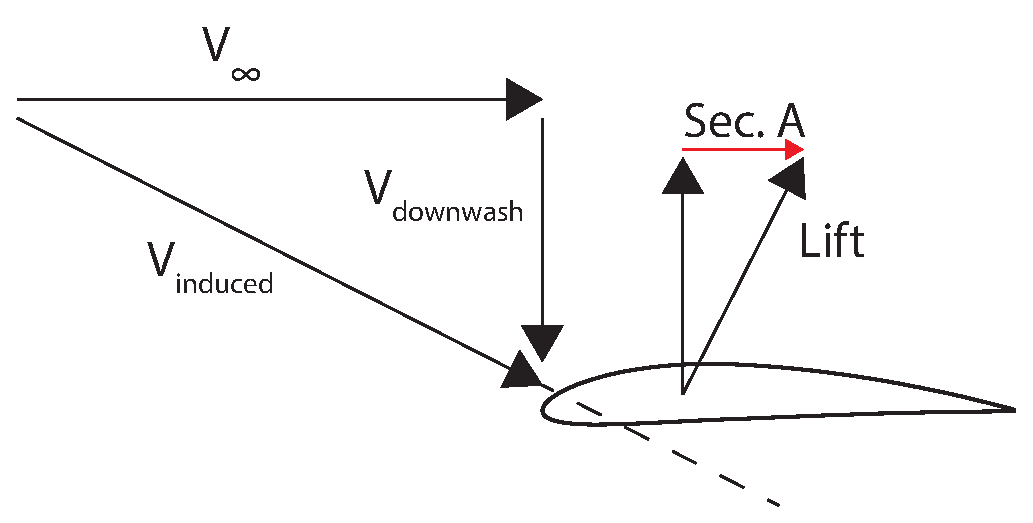
\includegraphics[width=.6\linewidth]{figures/inducedDrag.eps}
  \captionof{figure}{Induced Drag Free Body Diagram}
  \label{inducedDrag}
\end{figure}

The red section, labeled Sec. A in Figure \ref{inducedDrag}, is a component of the airfoil's lift which is parallel to $V_\infty$, meaning the airfoil's lift causes drag on the vehicle.\\

Induced drag is affected by the span lift distribution and the wing aspect ratio\cite{prandtl1923applications}, and is governed by Equation \ref{inducedDragEqn}.

\begin{align}
\label{inducedDragEqn}
C_{D_i} &= \frac{C^2_L}{\pi e AR} = K_2 C^2_L
\end{align}

These three coefficients ($C_{D_0},K_1$, and $K_2$) are combined to result in a parabolic drag polar of the form 

\begin{align}
\label{parabolicDragEqn}
C_D &= C_{D_{min}} + K_1(C_L-C_{L_{MIN}})^2 + K_2C^2_L
\end{align}
This drag polar gives valuable insight into how a vehicle will perform. The complete drag polar can be found using various regression techniques, discussed in the following sections.

\section{Regression Model - Least Squares Fit}
The standard model for a polynomial regression is

\begin{align}
\label{polyRegress}
\hat{y} &= \beta_0 + \beta_1x + \beta_2x^2+...
\end{align}

When Equation \ref{parabolicDragEqn} is expanded and like-terms of $C_L$ are combined, equation \ref{polyRegress} becomes
\begin{align}
C_D = (C_{D_{min}} + K_1 C_{L_{min}}) -2K_1C_{L_{min}}C_L+(K_1+K_2)C^2_L
\end{align}

The value $(C_{D_{min}}+K_1C_{L_{min}})$ is referred to as the parasite drag coefficient, and is represented by $C_{D_0}$\cite{raymer}.
These coefficients can be estimated using an Ordinary Least Squares fit. The Ordinary Least Squares problem statement is as follows
\begin{align}
\bar{A}\vec{x} &= \vec{b}
\end{align}
If $\bar{A}$ is an $m$x$n$ matrix of measured state data, $\vec{x}$ is an $n$x$1$ vector of correlation coefficients, and $\vec{b}$ is an $m$x$1$ vector of measured function data, the solution to the Ordinary Least Squares problem is 

\begin{align}
\bar{A}\vec{x}&=\vec{b}\\
\bar{A}^T\bar{A}\vec{x} &= \bar{A}^T\vec{b}\\
(\bar{A}^T\bar{A})^{-1}(\bar{A}^T \bar{A})\vec{x} &= (\bar{A}^T\bar{A})^{-1}\bar{A}^T\vec{b}\\
\bar{I}\vec{x} &=(\bar{A}^T\bar{A})^{-1}\bar{A}^T\vec{b}
\end{align}

When applied to estimating a parabolic drag polar, the $\bar{A}$ matrix becomes
\begin{align}
\bar{A}_{i,:} &= 
\begin{bmatrix}
1 & C_{L_i} & C^2_{L_i}
\end{bmatrix}
\end{align}
the $\vec{b}$ vector becomes

\begin{align}
\vec{b}_i &=
\begin{bmatrix}
C_{D_i}
\end{bmatrix}
\end{align}

and the $\vec{x}$ vector, which is the vector of interest, becomes
\begin{align}
\vec{x} &=
\begin{bmatrix}
C_{D_0} & -2K_1C_{L_{min}} & (K_1+K_2)
\end{bmatrix}^T
\end{align}

The coefficients $C_{D_0}$, $K_1$, and $K_2$ can then be found, assuming $C_{L_{min}}$ is known through wind tunnel testing, XFOIL, CFD, or other means.

\section{Regression Model - Kalman Filter}
The coefficients in question can also be estimated using an Extended Kalman filter. The system can again be described as 

\begin{align}
C_D &= C_{D_0}-2K_1C_{L_{min}}C_L+(K_1+K_2)C^2_L
\end{align}

For the Kalman filter regression, the state to be estimated are the coefficients $C_{D_0}$, $-2K_1C_{L_{min}}$, and $K_1+K_2$. For ease of notation, substitute

\begin{align}
C_1 &= -2K_1C_{L_{min}}\\
C_2 &= K_1+K_2
\end{align}Since the regression coefficients should not change, the state transition matrix is an identity matrix, leading to

\begin{align}
\hat{x}_k &= \begin{bmatrix}
C_{D_0} & C_1 & C_2
\end{bmatrix}\\
A &= \begin{bmatrix}
1&0&0\\0&1&0\\0&0&1
\end{bmatrix}
\end{align}


The measured data $z_k$ is a vector containing the lift and drag coefficients at the $k$-th instant in time

\begin{align}
z_k &= \begin{bmatrix}
C_D\\C_L
\end{bmatrix} = h(x_{k},0)
\end{align}


The vector $y_k$ contains the estimates of $C_D$ and $C_L$ found using the \textit{a priori} state vector $\hat{x}^-_k$ and is equal to

\begin{align}
y_k &= \begin{bmatrix} C^-_{D_{0_k}}+C^-_{1_k}C_L+C^-_{2_k}C^2_L \\ C_L \end{bmatrix} =h(x^-_k,z_k,0)
\end{align}


To implement into the Extended Kalman filter, the Jacobian of $h(x^-_k,z_k,0)$ with respect to $x_k$ needs to be calculated. Once done, the $H$ matrix in the EKF becomes

\begin{align}
H_k = \begin{bmatrix}
1 & C_L & C^2_L\\0&0&0
\end{bmatrix}
\end{align}


With the $H$ matrix calculated, the EKF algorithim can be implemented as described in Section \ref{EKFTheory}. The measurement noise covariance at each instant was calculated by doing error propagation as described in Section \ref{pointErrorSection} and the process noise covariance was set to zero because the coefficients should be exactly constant.
